%%% TikZ Euclid Examples
%%% Author: Ada Huang <ada.zan.huang@gmail.com>
%%% License: MIT

\documentclass{article}

\usepackage{tikz}
\usepackage{tkz-euclide}
\usepackage{tkzexample}

\usepackage[dvipsnames]{xcolor}
\definecolor{ZBlue}             {RGB}{61,109,240}
\usepackage[
  breaklinks=true,
  colorlinks,
  citecolor=MarkLeachBlue,
  filecolor=MarkLeachBlue,
  linkcolor=ZBlue,
  urlcolor=ZBlue,
  bookmarksopen,
  %pdfstartview=FitW
]{hyperref}

\usepackage{gensymb} % \degree

%%% serif
% \RequirePackage[T1]{fontenc}
% \RequirePackage{newpxtext,eulerpx}
%%% sans
\renewcommand*\familydefault{\sfdefault}
\usepackage[OT1]{fontenc}
\usepackage[default]{raleway}
\usepackage{newtxsf}

\tikzset{%
  point style/.style = {%
    shape = circle,
    fill = black,
    inner sep = 0pt,
    outer sep = 0pt,
    minimum size = 2pt,
  }
}
\addtolength{\textwidth}{2cm}
\addtolength{\hoffset}{-1cm}

\begin{document}
\begin{center}
  \textcolor{MidnightBlue}{\Huge tkz-euclide examples}
\end{center}
\clearpage
\section{Points}

\subsection{Fixed Points}

\subsubsection{Cartesian Coordinates: \texttt{(x, y)}}

\begin{tkzexample}[latex=5cm,small]
  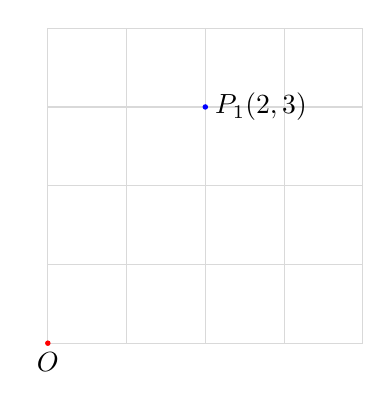
\begin{tikzpicture}
    \tkzInit[xmax=4,ymax=4]
    \tkzGrid[color=gray!30]
    \tkzDefPoint(0,0){O}
    \tkzDrawPoint[red](O)
    \tkzDefPoint(2,3){P1}
    \tkzDrawPoint[blue](P1)
    \tkzLabelPoint[right](P1){$P_1(2,3)$}
    \tkzLabelPoints[below](O)
  \end{tikzpicture}
\end{tkzexample}

\begin{tkzexample}[latex=5cm,small]
  \begin{tikzpicture}
    \tkzDefPoint(0,0){A}
    \tkzDefPoint(4,0){B}
    \tkzDefPoint(0,3){C}
    \tkzDrawPolygon(A,B,C)
    \tkzDrawPoints(A,B,C)
    \tkzLabelPoints[below](A,B)
    \tkzLabelPoints[above](C)
  \end{tikzpicture}
\end{tkzexample}

\subsubsection{Polar Coordinates: \texttt{(degree:radius)}}
\begin{tkzexample}[latex=5cm,small]
  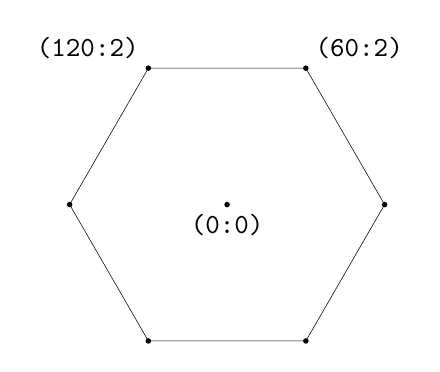
\begin{tikzpicture}
    \tkzDefPoint(0:0){O}
    \tkzDefPoint(60:2){A_1}  \tkzDefPoint(120:2){A_2}
    \tkzDefPoint(180:2){A_3} \tkzDefPoint(240:2){A_4}
    \tkzDefPoint(300:2){A_5} \tkzDefPoint(360:2){A_6}
    \tkzDrawPolygon(A_1,A_...,A_6)
    \tkzDrawPoints(A_1,A_...,A_6,O)
    \tkzLabelPoint[above right](A_1){\texttt{(60:2)}}
    \tkzLabelPoint[above left](A_2){\texttt{(120:2)}}
    \tkzLabelPoint[below](O){\texttt{(0:0)}}
  \end{tikzpicture}
\end{tkzexample}

\subsubsection{Multiple Points: \texttt{\textbackslash tkzDefPoints}}

\begin{tkzexample}[latex=5cm,small]
  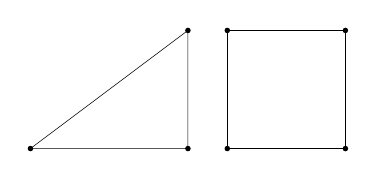
\begin{tikzpicture}[scale=1]
    \tkzDefPoints{0/0/A,2/0/B,2/1.5/C}
    \tkzDrawPolygon(A,B,C)
    \tkzDrawPoints(A,B,C)
    \tkzDefPoints{2.5/0/A,4/0/B,4/1.5/C,2.5/1.5/D}
    \tkzDrawPolygon(A,...,D)
    \tkzDrawPoints(A,B,C,D)
  \end{tikzpicture}
\end{tkzexample}

\subsection{Calculations: \href{https://ctan.org/pkg/xfp?lang=en}{\texttt{xfp}}}

\begin{tkzexample}[latex=5cm,small]
  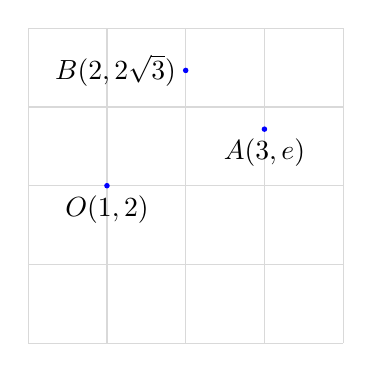
\begin{tikzpicture}
    \tkzInit[xmax=4,ymax=4] \tkzGrid[color=gray!30]
    \tkzDefPoint(-1+2,sqrt(4)){O}
    \tkzDefPoint({3*ln(exp(1))},{exp(1)}){A}
    \tkzDefPoint({4*sin(pi/6)},{4*cos(pi/6)}){B}
    \tkzDrawPoints[color=blue](O,B,A)
    \tkzLabelPoint[below](O){$O(1,2)$}
    \tkzLabelPoint[below](A){$A(3,e)$}
    \tkzLabelPoint[left](B){$B(2,2\sqrt{3})$}
  \end{tikzpicture}
\end{tkzexample}

\subsection{Point Relative to Another: \texttt{\textbackslash tkzDefShiftPoint}}

\begin{tkzexample}[latex=5cm,small]
  \begin{tikzpicture}[scale=1]
    \tkzDefPoint(2,3){A}
    \tkzDefShiftPoint[A](30:3){B}
    \tkzDefShiftPoint[A]({3/2*sqrt(3)},-1.5){C}
    \tkzDrawPolygon(A,B,C)
    \tkzDrawPoints(A,B,C)
    \tkzLabelPoints[right](B,C)
    \tkzLabelPoints[left](A)
    \tkzMarkSegments[mark=||,color=red](A,B A,C B,C)
  \end{tikzpicture}
\end{tkzexample}

\subsection{Midpoint: \texttt{\textbackslash tkzDefMidPoint}}

\begin{tkzexample}[latex=5cm,small]
  \begin{tikzpicture}[scale=1]
    \tkzDefPoint(2,3){A}
    \tkzDefPoint(4,0){B}
    \tkzDefMidPoint(A,B) \tkzGetPoint{C}
    \tkzDrawSegment(A,B)
    \tkzDrawPoints(A,B,C)
    \tkzLabelPoints[right](A,B,C)
  \end{tikzpicture}
\end{tkzexample}

\subsection{Barycenter: \texttt{\textbackslash tkzDefBarycentricPoint}}

\begin{tkzexample}[latex=5cm,small]
  \begin{tikzpicture}
    \tkzDefPoint(1,1.5){A}
    \tkzDefShiftPointCoord[1,1.5](15:3.2){B}
    \tkzDefBarycentricPoint(A=2,B=5)
    \tkzGetPoint{I}
    \tkzDrawPoints(A,B,I) \tkzDrawLine(A,B)
    \tkzLabelPoints(A,B,I)
  \end{tikzpicture}
\end{tkzexample}

\subsection{Point on a Line: \texttt{\textbackslash tkzDefPointOnLine}}

\begin{tkzexample}[latex=4cm,small]
  \begin{tikzpicture}
    \tkzDefPoints{0/0/A,1/3/B}
    \tkzDrawLine[red](A,B)
    \tkzDefPointOnLine[pos=1.2](A,B)  \tkzGetPoint{P}
    \tkzDefPointOnLine[pos=-0.2](A,B) \tkzGetPoint{R}
    \tkzDefPointOnLine[pos=2/3](A,B)  \tkzGetPoint{S}
    \tkzLabelPoints[right](A,B)
    \tkzLabelPoint[left](P){$P$ (pos=$1.2$)}
    \tkzLabelPoint[left](R){$R$ (pos=$-.2$)}
    \tkzLabelPoint[left](S){$S$ (pos=$\dfrac{2}{3}$)}
    \tkzDrawPoints(A,B,P,R,S)
  \end{tikzpicture}
\end{tkzexample}

\subsection{Point on a Circle: \texttt{\textbackslash tkzDefPointOnCircle}}

\begin{tkzexample}[latex=4cm,small]
  \begin{tikzpicture}[scale=0.7]
    \tkzDefPoints{0/0/A,4/0/B,0.8/3/C}
    \tkzDefCircle[circum](A,B,C)
    \tkzGetPoint{O} \tkzGetLength{rO}
    \tkzDefPointOnCircle[R=center O angle 30 radius \rO]
    \tkzGetPoint{J}
    \tkzDrawPoints(A,B,C)
    \tkzDrawCircle(O,J)
    \tkzDrawPoints(O,J)
    \tkzDrawPoint[red](J)
    \tkzLabelPoints[right](O,J)
  \end{tikzpicture}
\end{tkzexample}

\subsection{Transformations: \texttt{\textbackslash tkzDefPointBy}}

\subsubsection{Translation}

\begin{tkzexample}[latex=4cm,small]
  \begin{tikzpicture}[>=latex]
    \tkzDefPoints{0/0/A, 1/2/B, 2/1/B'}
    \tkzDefPointBy[translation= from B to A](B')
    \tkzGetPoint{A'}
    \tkzDrawPoints[teal](A,B,A',B')
    \tkzLabelPoints[above, color=teal](B,B')
    \tkzLabelPoints[below, color=teal](A,A')
    \tkzDrawSegments[orange,->](A,B A',B')
  \end{tikzpicture}
\end{tkzexample}

\subsubsection{Reflection}
\begin{tkzexample}[latex=5cm,small]
  \begin{tikzpicture}
    \tkzDefPoints{0/0/X,4/4/Y,2/1/A,4/2/B,2.5/0/C}
    \tkzDrawSegment(X,Y)
    \tkzDefPointBy[reflection=over X--Y](A)
    \tkzGetPoint{A'}
    \tkzDefPointBy[reflection=over X--Y](B)
    \tkzGetPoint{B'}
    \tkzDefPointBy[reflection=over X--Y](C)
    \tkzGetPoint{C'}
    \tkzDrawPoints(A,B,C,A',B',C')
    \tkzDrawPolygons(A,B,C A',B',C')
  \end{tikzpicture}
\end{tkzexample}

\subsubsection{Projection}

\begin{tkzexample}[latex=5cm,small]
  \begin{tikzpicture}
    \tkzDefPoints{0/0/A,4/1/B,3/2/C}
    \tkzDrawSegment(A,B)
    \tkzDefPointBy[projection=onto A--B](C)
    \tkzGetPoint{D}
    \tkzDrawPoints(A,B,C,D)
    \tkzDrawSegment[densely dashed](C,D)
    \tkzMarkRightAngle[size=.2](B,D,C)
    \tkzLabelPoints(A,B,D)
    \tkzLabelPoints[right](C)
  \end{tikzpicture}
\end{tkzexample}

\subsubsection{Symmetry}

\begin{tkzexample}[latex=5cm,small]
  \begin{tikzpicture}[scale=1]
    \tkzDefPoint(0,0){O}
    \tkzDefPoint(1.5,-1){A}
    \tkzDefPoint(2,1){B}
    \tkzDefPointsBy[symmetry=center O](B,A){}
    \tkzDrawSegments[densely dashed](A,A' B,B')
    \tkzDrawPoints(A,B,O,A',B')
    \tkzLabelPoints[below](A,B')
    \tkzLabelPoints[above](A',O,B)
  \end{tikzpicture}
\end{tkzexample}

\subsubsection{Rotation and Rotation in Rad}

\begin{tkzexample}[latex=5cm,small]
  \begin{tikzpicture}
    \tkzDefPoint["$A$" left](0,0){A}
    \tkzDefPoint["$B$" right](3,0){B}
    \tkzDefPointBy[rotation=center A angle 60](B)
    \tkzGetPoint{C}
    \tkzDefPointBy[rotation in rad=center A angle -pi/3](B)
    \tkzGetPoint{C'}
    \tkzLabelPoints[right](C,C')
    \tkzDrawPoints(A,B,C,C')
    \tkzDrawSegments(A,B A,C A,C')
    \tkzMarkAngles[mark=none, size=0.4cm](B,A,C C',A,B)
    \tkzLabelAngles[pos=0.75](B,A,C C',A,B){$60\degree$}
    \tkzMarkSegments[mark=||](A,B A,C A,C')
  \end{tikzpicture}
\end{tkzexample}

\subsection{Defining Points Using a Vector: \texttt{\textbackslash tkzDefPointWith}}

\subsubsection{Linear}

\begin{tkzexample}[latex=5cm,small]
  \begin{tikzpicture}
    \tkzDefPoint(1,3){A}
    \tkzDefPoint(4,2){B}
    \tkzDefPointWith[linear,K=2/3](A,B)
    \tkzGetPoint{C}
    \tkzDrawPoints[color=red](A,B,C)
    \tkzDrawSegment(A,B)
    \tkzLabelPoints[above right=3pt](A,B,C)
  \end{tikzpicture}
\end{tkzexample}

\subsubsection{Colinear}

\begin{tkzexample}[latex=5cm,small]
  \begin{tikzpicture}[scale=1.2,
      vect/.style={->,shorten >=3pt,>=latex'}]
    \tkzDefPoint(2,3){A}
    \tkzDefPoint(4,2){B}
    \tkzDefPoint(1,2){C}
    \tkzDefPointWith[colinear=at C](A,B)
    \tkzGetPoint{D}
    \tkzDrawPoints[color=red](A,B,C,D)
    \tkzLabelPoints[above right=3pt](A,B,C,D)
    \tkzDrawSegments[vect](A,B C,D)
  \end{tikzpicture}
\end{tkzexample}

\begin{tkzexample}[latex=5cm,small]
  \begin{tikzpicture}[scale=1.2,
      vect/.style={->,shorten >=3pt,>=latex'}]
    \tkzDefPoints{2/3/A, 4/2/B}
    \tkzDefPointWith[orthogonal,K=2/3](A,B)
    \tkzGetPoint{C}
    \tkzDefPointWith[orthogonal,normed,K=-1](B,A)
    \tkzGetPoint{D}
    \tkzDrawPoints[color=red](A,B,C,D)
    \tkzLabelPoints[right=3pt](B,C,D)
    \tkzLabelPoints[below=3pt](A)
    \tkzDrawSegments[vect](A,B A,C B,D)
    \tkzMarkRightAngle(B,A,C)
  \end{tikzpicture}
\end{tkzexample}

\subsection{Triangle Centers: \texttt{\textbackslash tkzDefTriangleCenter}}

\subsubsection{Centroid}

\begin{tkzexample}[latex=5cm,small]
  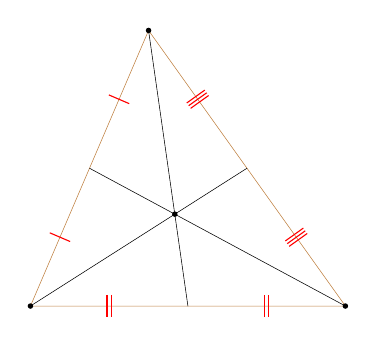
\begin{tikzpicture}
    \tkzDefPoints{0/0/A,4/0/B,1.5/3.5/C}
    \tkzDrawPolygon[color=brown](A,B,C)
    \tkzDefTriangleCenter[centroid](A,B,C) \tkzGetPoint{D}
    \tkzDrawPoints(A,B,C,D)
    \tkzDefMidPoint(A,B) \tkzGetPoint{E}
    \tkzDefMidPoint(B,C) \tkzGetPoint{F}
    \tkzDefMidPoint(C,A) \tkzGetPoint{G}
    \tkzDrawSegments(C,E A,F B,G)
    \tkzMarkSegments[mark=|,color=red](C,G A,G)
    \tkzMarkSegments[mark=||,color=red](A,E B,E)
    \tkzMarkSegments[mark=|||,color=red](B,F C,F)
  \end{tikzpicture}
\end{tkzexample}

\subsubsection{Incenter}

\begin{tkzexample}[latex=5cm,small]
  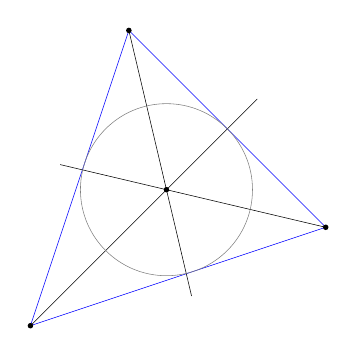
\begin{tikzpicture}[scale=1.25]
    \tkzDefPoints{0/1/A,3/2/B,1/4/C}
    \tkzDefTriangleCenter[in](A,B,C) \tkzGetPoint{I}
    \tkzDefPointBy[projection=onto A--C](I)
    \tkzGetPoint{Ib}
    \tkzDrawPolygon[color=blue](A,B,C)
    \tkzDrawPoints(A,B,C,I)
    \tkzDrawLines[add = 0 and 2/3](A,I B,I C,I)
    \tkzDrawCircle(I,Ib)
  \end{tikzpicture}
\end{tkzexample}

\subsubsection{Circumcenter}

\begin{tkzexample}[latex=5cm,small]
  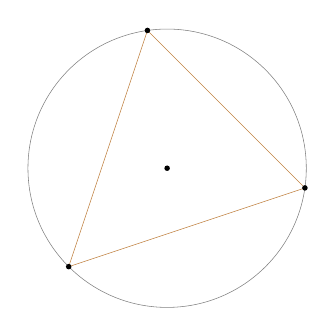
\begin{tikzpicture}
    \tkzDefPoints{0/1/A,3/2/B,1/4/C}
    \tkzDefTriangleCenter[circum](A,B,C) \tkzGetPoint{G}
    \tkzDrawPolygon[color=brown](A,B,C)
    \tkzDrawCircle(G,A)
    \tkzDrawPoints(A,B,C,G)
  \end{tikzpicture}
\end{tkzexample}

\subsubsection{Orthocenter}

\begin{tkzexample}[latex=5cm,small]
  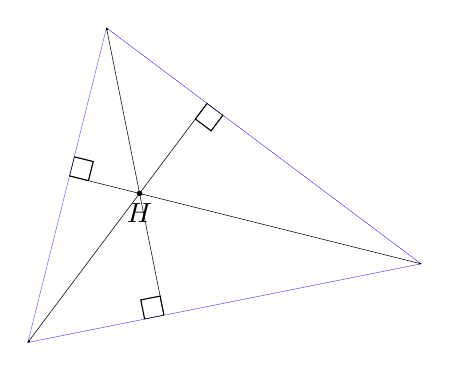
\begin{tikzpicture}
    \tkzDefPoint(0,0){A}
    \tkzDefPoint(5,1){B}
    \tkzDefPoint(1,4){C}
    \tkzClipPolygon(A,B,C)
    \tkzDefTriangleCenter[ortho](B,C,A) \tkzGetPoint{H}
    \tkzDefSpcTriangle[orthic,name=H](A,B,C){a,b,c}
    \tkzDrawPolygon[color=blue](A,B,C)
    \tkzDrawPoints(A,B,C,H)
    \tkzDrawLines[add=0 and 1](A,Ha B,Hb C,Hc)
    \tkzLabelPoint(H){$H$}
    \tkzAutoLabelPoints[center=H](A,B,C)
    \tkzMarkRightAngles(A,Ha,B B,Hb,C C,Hc,A)
  \end{tikzpicture}
\end{tkzexample}

\subsubsection{Excenter}

\begin{tkzexample}[latex=5cm,small]
  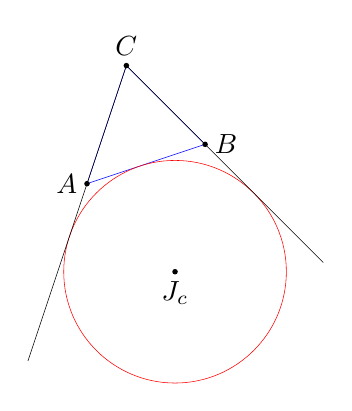
\begin{tikzpicture}[scale=0.5]
    \tkzDefPoints{0/1/A,3/2/B,1/4/C}
    \tkzDefTriangleCenter[ex](B,C,A) \tkzGetPoint{J_c}
    \tkzDefPointBy[projection=onto A--B](J_c)
    \tkzGetPoint{Tc}
    \tkzDrawPolygon[color=blue](A,B,C)
    \tkzDrawPoints(A,B,C,J_c)
    \tkzDrawCircle[red](J_c,Tc)
    \tkzDrawLines[add=1.5 and 0](A,C B,C)
    \tkzLabelPoints[left](A)
    \tkzLabelPoints[right](B)
    \tkzLabelPoints[above](C)
    \tkzLabelPoints(J_c)
  \end{tikzpicture}
\end{tkzexample}

\section{Lines}

\subsection{Definition: \texttt{\textbackslash tkzDefLine}}

\subsubsection{Mediator}

\begin{tkzexample}[latex=5cm,small]
  \begin{tikzpicture}[scale=0.7]
    \tkzSetUpPoint[size=1.5pt]
    \tkzDefPoints{-2/0/A,1/2/B}
    \tkzDefLine[mediator](A,B)
    \tkzGetPoints{C}{D}
    \tkzInterLL(C,D)(A,B)
    \tkzGetPoint{I}
    \tkzDrawPoints(A,B)
    \tkzDrawSegments(A,B C,D)
    \tkzMarkRightAngle[size=.2](A,I,C)
    \tkzMarkSegments[mark=||](A,I B,I)
  \end{tikzpicture}
\end{tkzexample}

\subsubsection{Bisector}

\begin{tkzexample}[latex=5cm,small]
  \begin{tikzpicture}[rotate=25,scale=.7]
    \tkzDefPoints{0/0/C, 2/-3/A, 4/0/B}
    \tkzDefLine[bisector,K=.5](B,A,C)
    \tkzGetPoint{a}
    \tkzDrawLines[add= 0 and .5](A,B A,C)
    \tkzShowLine[bisector,gap=4,size=2,color=red](B,A,C)
    \tkzDrawLines[blue!50,dashed,add= 0 and .5](A,a)
    \tkzLabelPoints[below](A,C)
    \tkzLabelPoints[right](B)
    \tkzDrawPoints[size=1.5pt](A,B,C,a)
  \end{tikzpicture}
\end{tkzexample}

\subsubsection{Orthogonal And Parallel}

\begin{tkzexample}[latex=5cm,small]
  \begin{tikzpicture}
    \tkzDefPoints{-1.5/-0.25/A,1/-0.75/B,-0.7/1/C}
    \tkzDrawLine(A,B)
    \tkzDefLine[orthogonal=through C](B,A)
    \tkzGetPoint{c}    \tkzDrawLine(C,c)
    \tkzInterLL(A,B)(C,c)    \tkzGetPoint{I}
    \tkzDefLine[parallel=through C](A,B)
    \tkzGetPoint{D}    \tkzDrawLine(C,D)
    \tkzDrawPoints(A,B,C,c,D)
    \tkzLabelPoints[above right](A,B,C,c,D)
    \tkzLabelLine[pos=1.25,below left](A,B){$(l_1)$}
    \tkzLabelLine[pos=1.2,right](C,D){$(l_2)$}
    \tkzLabelLine[pos=1.25,left](C,c){$\delta$}
    \tkzMarkRightAngle(C,I,B)\tkzMarkRightAngle(I,C,D)
  \end{tikzpicture}
\end{tkzexample}

\subsection{Tangent to a Circle: \texttt{\textbackslash tkzDefTangent}}

\begin{tkzexample}[latex=5cm,small]
  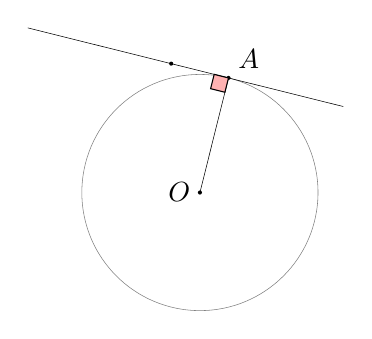
\begin{tikzpicture}[scale=.75]
    \tkzDefPoint(0,0){O}
    \tkzDefRandPointOn[circle=center O radius 2]
    \tkzGetPoint{A}
    \tkzDrawSegment(O,A)
    \tkzDrawCircle(O,A)
    \tkzDefTangent[at=A](O)    \tkzGetPoint{h}
    \tkzDrawPoints[size=1.5pt](A,O,h)
    \tkzDrawLine[add = 2 and 2.5](A,h)
    \tkzMarkRightAngle[fill=red!30](O,A,h)
    \tkzLabelPoints[above right](A) \tkzLabelPoints[left](O)
  \end{tikzpicture}
\end{tkzexample}

\subsection{Median, Altitude, and Bisector}

\begin{tkzexample}[latex=5cm,small]
  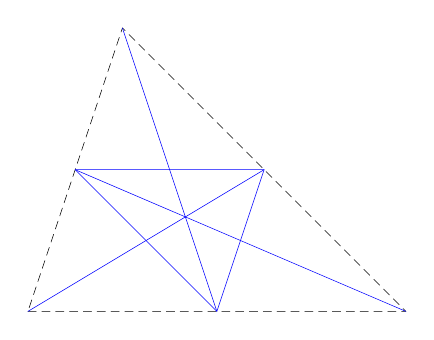
\begin{tikzpicture}[scale=1.2]
    \tkzDefPoint(0,0){A}
    \tkzDefPoint(4,0){B}
    \tkzDefPoint(1,3){C}
    \tkzDrawPolygon[densely dashed](A,B,C)
    \tkzSetUpLine[color=blue]
    \tkzDefSpcTriangle[medial,name=M](A,B,C){_A,_B,_C}
    \tkzDrawSegments(A,M_A B,M_B C,M_C)
    \tkzDrawPolygon(M_A, M_B, M_C)
  \end{tikzpicture}
\end{tkzexample}

\begin{tkzexample}[latex=5cm,small]
  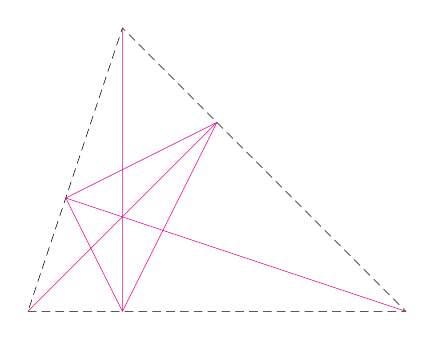
\begin{tikzpicture}[scale=1.2]
    \tkzDefPoint(0,0){A}
    \tkzDefPoint(4,0){B}
    \tkzDefPoint(1,3){C}
    \tkzDrawPolygon[densely dashed](A,B,C)
    \tkzSetUpLine[color=magenta]
    \tkzDefSpcTriangle[orthic,name=H](A,B,C){_A,_B,_C}
    \tkzDrawSegments(A,H_A B,H_B C,H_C)
    \tkzDrawPolygon(H_A, H_B, H_C)
  \end{tikzpicture}
\end{tkzexample}

\begin{tkzexample}[latex=5cm,small]
  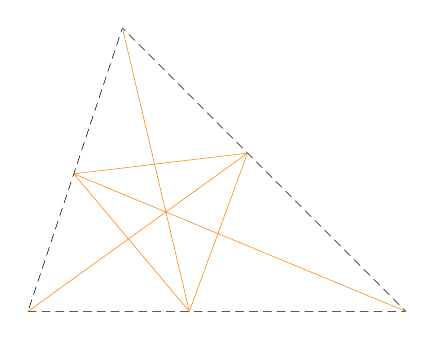
\begin{tikzpicture}[scale=1.2]
    \tkzDefPoint(0,0){A}
    \tkzDefPoint(4,0){B}
    \tkzDefPoint(1,3){C}
    \tkzDrawPolygon[densely dashed](A,B,C)
    \tkzSetUpLine[color=orange]
    \tkzDefSpcTriangle[in,name=I](A,B,C){_A,_B,_C}
    \tkzDrawSegments(A,I_A B,I_B C,I_C)
    \tkzDrawPolygon(I_A, I_B, I_C)
  \end{tikzpicture}
\end{tkzexample}

\subsection{Drawing: \texttt{\textbackslash tkzDrawSegment and \textbackslash tkzDrawLine}}

\begin{tkzexample}[latex=5cm,small]
  \begin{tikzpicture}[scale=1.5]
    \tkzDefPoint(0,0){A}
    \tkzDefPoint(2,1){B}
    \tkzDrawSegment[color=red,thin](A,B)
    \tkzDrawPoints(A,B)
    \tkzLabelPoints(A,B)
 \end{tikzpicture}
\end{tkzexample}

\begin{tkzexample}[latex=5cm,small]
  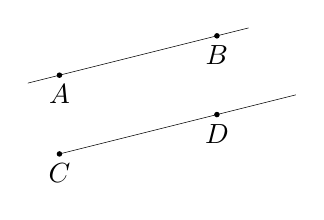
\begin{tikzpicture}
    \tkzDefPoint(0,0){A}
    \tkzDefPoint(2,0.5){B}
    \tkzDefPoint(0,-1){C}\tkzDefPoint(2,-0.5){D}
    \tkzDrawLine(A,B)
    \tkzDrawLine[add = 0 and .5](C,D)
    \tkzDrawPoints(A,B,C,D) \tkzLabelPoints(A,B,C,D)
  \end{tikzpicture}
\end{tkzexample}

\begin{tkzexample}[latex=5cm,small]
  \begin{tikzpicture}
    \tkzDefPoint(0,0){A}
    \tkzDefPoint(2,0){B}
    \tkzDefPoint(1,2){C}
    \tkzDefPoint(3,2){D}
    \tkzDrawLines(A,B C,D A,C B,D)
    \tkzLabelPoints[below right](A,B,C,D)
  \end{tikzpicture}
\end{tkzexample}

\subsubsection{Labeling: \texttt{\textbackslash tkzLabelLine}}

\begin{tkzexample}[latex=5cm,small]
  \begin{tikzpicture}[scale=0.8]
    \tkzDefPoints{0/0/A,3/0/B,1/1/C}
    \tkzDefLine[perpendicular=through C,K=-1](A,B)
    \tkzGetPoint{c}
    \tkzDrawLines(A,B C,c)
    \tkzLabelLine[pos=1.25,blue,right](C,c){$l_1$}
    \tkzLabelLine[pos=-0.25,red,above](A,B){$l_2$}
  \end{tikzpicture}
\end{tkzexample}

\begin{tkzexample}[latex=5cm,small]
  \begin{tikzpicture}
    \tkzDefPoint(0,0){A}
    \tkzDefPoint(4,0){B}
    \tkzDefTriangle[pythagore](A,B)  \tkzGetPoint{C}
    \tkzDrawPoints[size=1.5pt](A,B,C)
    \tkzDrawSegment[dim={$3$, 6pt, transform shape},
      dim style/.append style={blue}](B,C)
    \tkzDrawSegment[dim={$4$, 6pt, transform shape},
      dim style/.append style={densely dashed, red}](A,B)
    \tkzDrawSegment[dim={$5$, 1cm, transform shape},
      dim fence style/.style={red,densely dashed}](C,A)
    \tkzLabelPoints[left](A) \tkzLabelPoints[above right](B)
    \tkzLabelPoints[below](C)
  \end{tikzpicture}
\end{tkzexample}

\subsubsection{Marking: \texttt{\textbackslash tkzMarkSegment}}

\begin{tkzexample}[latex=5cm,small]
  \begin{tikzpicture}
    \tkzDefPoint(2,1){A}
    \tkzDefPoint(6,4){B}
    \tkzDrawSegment(A,B)
    \tkzMarkSegment[thick,color=gray,pos=0.2,mark=s|](A,B)
    \tkzMarkSegment[thick,color=gray,pos=0.4,mark=s||](A,B)
    \tkzMarkSegment[thick,color=brown,pos=0.6,mark=||](A,B)
    \tkzMarkSegment[thick,color=red,pos=0.8,mark=|||](A,B)
  \end{tikzpicture}
\end{tkzexample}

\end{document}
